\documentclass[12pt,oneside,final]{fithesis2}
\usepackage[czech]{babel}
\usepackage[utf8]{inputenc}
\usepackage[T1]{fontenc}
\usepackage[plainpages=false,pdfpagelabels,unicode]{hyperref}
\usepackage[pdftex]{graphicx}
\usepackage{tikz}
\usepackage[version=3]{mhchem}
\usepackage[total={16.5cm,25cm}, top=3cm, left=3cm, includefoot]{geometry}%nalevo3 napravo 1,5

\thesistitle{Plazmochemická depozice tenkých vrstev a jejich optické vlastnosti v UV až IR oblasti}
\thesissubtitle{Bakalářská práce}
\thesisstudent{Pavel Ondračka}
\thesiswoman{false}
\thesisfaculty{sci}
\thesisyear{jaro 2011}
\thesisadvisor{doc. Mgr. Lenka Zajíčková, Ph.D.}
\thesislang{cs}

\begin{document}
\FrontMatter
\ThesisTitlePage

\begin{ThesisDeclaration}
\DeclarationText
\AdvisorName
\end{ThesisDeclaration}

\begin{ThesisThanks}
Děkuji vedoucí práce doc. Mgr. Lence Zajíčkové Ph.D. za uvedení do problematiky, časté konzultace a opravy práce, Mgr. Danielu Frantovi, Ph.D. a Mgr. Davidu Nečasovi za rady ke zpracování dat a optickým měřením a Mihai George Muresanovi, M.Sc. za pomoc při depozici vrstev.
\end{ThesisThanks}

\begin{ThesisAbstract}
Během této práce byly nanášeny tenké vrstvy ve vysokofrekvenčním doutnavém výboji ze směsi hexametyldisiloxanu a kyslíku. Dále byly měřeny optické vlastnosti připravených vrstev. Za tímto účelem byla použita spektroskopická elipsometrie a odrazivost v~oblasti ultrafialového (UV) až viditelného záření a měření transmise v infračervené oblasti. Byly zkoumány vlivy depozičních podmínek na optické vlastnosti, rychlost depozice a chemické složení vrstev.
\\
\\
\\
{\large \bf Klíčová slova}
\\
\\
PECVD, HMDSO, plazmová polymerace, plazma, tenké vrstvy
\\
\\
\\
{\Large \bf Abstract}
\\
\\
In this thesis, thin films were deposited from the mixture of oxygen and hexamethyldisiloxane in radio frequency glow discharge. The optical properties of the deposited films were measured by spectroscopic ellipsometry and reflectance in ultraviolet and visible range. Chemical structure of the films was studied by transmittance in infrared range. The influence of deposition parameters for optical constants, deposition speed and chemical composition of film were examined. 
\\
\\
\\
{\large \bf Keywords}
\\
\\
PECVD, HMDSO, plasma polymerization, plasma, thin films

\end{ThesisAbstract}



\MainMatter

\tableofcontents % prints table of contents

\chapter{Úvod}
Plazmochemická depozice vrstev z plynné fáze (PECVD\footnote{Plasma-enhanced chemical vapor deposition}) skýtá zajímavé možnosti z hlediska přípravy nových materiálů. Změnou parametrů výboje je možné podstatně ovlivnit podmínky depozice a tím i vlastnosti připravených vrstev. Optické metody charakterizace tenkých vrstev, tedy elipsometrie a spektrofotometrie, poskytují celou řadu informací o vlastnostech vrstev. V oblasti ultrafialového (UV) až viditelného záření jsou důležité pro mnohé aplikace jejich optické konstanty (index lomu a extinkční koeficient). Je rovněž možné zjistit jejich tloušťku, a tedy depoziční rychlost, což je důležité pro průmyslové aplikace. V infračervené oblasti poskytuje absorpce ve vrstvách informace o chemických vazbách, tudíž i o složení a struktuře vrstev.


\chapter{PECVD}

Plazmochemická depozice z plynné fáze (PECVD) je proces využívaný k depozici tenkých vrstev z plynné fáze na substrát. Zatímco při chemické depozici (CVD\footnote{Chemical vapor deposition}) je aktivační energie reakcí v plynu a na substrátu získána díky vysoké teplotě, v PECVD je využito plazmatu k vyvolání chemických reakcí při nízkých teplotách. Běžné energie elektronů při nízkotlakových výbojích jsou kolem 2--5\,eV, což dostačuje pro disociaci neutrálních molekul plynu, zatímco substrát a těžké částice mají teplotu mnohem menší. 
 
Mimo to je v metodě PECVD často využíváno i iontové bombardování rostoucí vrstvy. Využití iontového bombardování může zlepšit elektrické a mechanické vlastnosti a vést ke zvýšení hustoty a tvrdosti tenké vrstvy. Kromě toho se iontové bombardování využívá před depozicí k odstranění nečistoty na substrátu a ke zvýšení adheze vrstvy \cite{smith, liebermanPECVD}. 

\section{Plazmová polymerizace}

Plazmová polymerizace označuje PECVD proces, při kterém se na povrchu substrátu vytváří organický polymer. Od jiných polymerů, vzniklých mimo plazmu, se liší tím, že nemá žádnou rozpoznatelnou pravidelně se opakující jednotku. Plazmový polymer je typicky vysoce větvený a zesíťovaný. Jeho vlastnosti závisí jednak na použitém monomeru a často velmi silně i na parametrech plazmatu \cite{yasudapoly}.
 
Při depozicích byl použit hexametyldisiloxan (HMDSO), což je organosilikonová sloučenina s chemickým vzorcem  \ce{O(Si(CH3)3)2}. HMDSO je často využíván při plazmové polymeraci kvůli jeho vysoce organickému charakteru a vysoké tenzi par. Při PECVD se používá samostatně, případně ve směsi s kyslíkem, argonem, metanem nebo vodíkem. V~současné době je hojně využíván pro ochranné povrchy na plastové substráty, bariérové fólie na potraviny a farmaceutická balení, ochranu proti korozi vrstvy, povlaky pro~biokompatibilní materiály, low-k dielektrické vrstvy pro mikroelektronické aplikace a mnoho dalších aplikací \cite{zajickova2007}. Vlastnosti vrstvy se odvíjí od množství HMDSO. Organosilikonové plazmové polymery připravujeme depozicí z čistého HMDSO, případně s příměsí neoxidujícího plynu, nebo s malou příměsí oxidantu. Anorganické \ce{SiO2} podobné vrstvy se dají připravit z HMDSO vysoce zředěného v kyslíku \cite{zajickova2007b}. 



\chapter{Plazma}

Pojem plazma můžeme použít pro makroskopicky neutrální látku, která obsahuje velké množství interagujících volných elektronů a ion\-tů, vykazuje kolektivní chování díky dalekodosahovým coulombov\-ským silám a splňuje následující kritéria \cite{bittencourtplasmadef}:

\begin{enumerate}

\item {V médiu musí být dostatek prostoru pro kolektivní stínící efekt:
	\begin{equation} L \ll \lambda_D \mathrm{,}\end{equation}
	kde L jsou fyzikální rozměry plazmatu a $\lambda_D$ je debyeovská délka plazmatu (míra vzdálenosti na kterou je nabitá částice odstíněna, díky 		kolektivnímu chování částic, od jiné nabité částice nebo plochy s nenulovým potenciálem):
	\begin{equation} \lambda_D = \sqrt{\frac{\epsilon_0 k T}{n_e e^2}} \mathrm{,}\end{equation}
	$\epsilon_0$ je permitivita vakua, $k$ je Boltzmanova konstanta, $T$ je teplota, $n_e$ je hustota elektronů a $e$ je elementární náboj.	
	}

\item{Dostatečně velký počet částic uvnitř Debyeovy koule:
	\begin{equation} \lambda_D^3 n_e \gg 1 \mathrm{.}\end{equation}
     }

\item{Kvazineutralita\\ 
	V objemu, který je podstatně větší než debyeovská délka, musí být zachována rovnováha mezi koncentracemi kladných a záporných nositelů.}

\item{
	Srážky mezi elektrony a neutrály nesmí příliš tlumit plazmové oscilace.\\
	V plazmatu, v důsledku snahy o vyrovnání lokální nerovnováhy náboje, vznikají díky coulombovským silám kmity, které můžeme charakterizovat tzv. elektronovou plazmovou frekvencí:
	\begin{equation}\omega_{pe} = \sqrt\frac{n_e e^2}{m_e \epsilon_0} \mathrm{,}\end{equation}
	kde $m_e$ je hmotnost elektronu. Pro plazma musí platit: 
	\begin{equation}\frac{\omega_{pe}}{2 \pi} > \nu_{en} \mathrm{,}\end{equation}
	kde $\nu_{en}$ je srážková frekvence elektronů s neutrály.
	}

\end{enumerate} 



\section{Procesy v plazmatu}



\subsection {Srážky v plazmatu}
V plazmatu se nachází elektrony, ionty a neutrální molekuly. Srážky mezi nimi dělíme na~pružné a nepružné, podle toho zda se při nich zachovává celková kinetická energie částic. Při neelastických (nepružných) srážkách dochází k různým procesům \cite{chen2003reactions}. 

\begin{itemize}
  \item {Ionizace\\
	\ce{e- + A -> A+ + 2e-}\\
	Elektron s dostatečnou energií může vyrazit další elektron z atomu za vzniku iontu. Oba dva elektrony jsou opět urychlovány a ionizují další atomy. Toto je nejdůležitější děj pro zachování plazmatu.  }
  \item{Excitace\\
	\ce{e- + A -> A$^*$ + e-}\\
	 Při neelastické srážce elektronu s atomem může také dojít k excitaci valenčního elektronu na~vyš\-ší energetickou hladinu. Chemická reaktivita výsledného atomu je různá od reaktivity jeho základního stavu.}
  \item{Disociace\\
	\ce{e- + A2 -> e- + A. + A.}\\
	Při srážce elektronu s molekulou může dojít k rozbití chemické vazby. Podle energie reakce mohou být produkty v základním nebo excitovaném stavu. Obecně je energie potřebná pro disociaci menší než energie potřebná pro ionizaci. Většina chemicky aktivních radikálů v plazmatu vzniká tímto procesem.
 }
  \item{Deexcitace (fotoemise)\\
	\ce{A$^*$ -> A + $h\nu$}\\
	Excitované stavy atomů jsou většinou nestabilní a elektrony se brzo vrací do základního stavu. Přitom je vyzářen foton s energií odpovídající rozdílu mezi těmito dvěma stavy. Většina atomů zůstává v excitovaném stavu pouze asi $10^{-8}$\,s. Některé atomy mají tzv. metastabilní stavy, kde k deexcitaci dochází až po dlouhé době ($\sim$1--10\,ms). Příkladem atomů s metastabilními stavy jsou vzácné plyny.}
  \item{Rekombinace\\
	\ce{e- + A+ + A	-> A$^*$ + A}\\
	Při rekombinaci dochází k reakci mezi elektronem a iontem. Kvůli zachování energie a hybnosti musí být přítomen další reaktant. To je většinou neutrál, jehož je v~plazmatu dostatek, nebo může k reakci dojít na stěně reaktoru.}
  \item{Záchyt elektronu\\
	\ce{e- + A -> A-}\\
	Elektrony mohou být zachyceny na elektronegativních atomech za vzniku záporného iontu.
	}
  \item{Iontová rekombinace\\
	\ce{A+ + A- -> A + A}\\
	Pokud jsou v plazmatu přítomny záporné ionty, mají určitou (malou) pravděpodobnost srážky s kladným iontem. Dojde k přesunu elektronu a výsledek reakce jsou dva neutrály.}
  \item{Zářivá rekombinace\\
	\ce{e- + A+ -> A + $h\nu$}\\}
\end {itemize}

Uvedený seznam je jen souhrn nejjednodušších reakcí, které mohou nastat. Pro složitější molekuly a sloučeniny je možností řádově více. Například typickými reakcemi, které probíhají v HMDSO plazmatu, jsou:
\begin{eqnarray} \nonumber\lefteqn{\ce{(CH3)3SiOSi(CH3)3 + e-}}\\
&\ce{->}&\ce{(CH3)3Si + (CH3)3SiO+ + 2e-}\\  
&\ce{->}&\ce{(CH3)3Si+ + (CH3)3SiO + 2e-}\\
&\ce{->}&\ce{(CH3)3Si-O-Si+(CH3)2 + CH3 + 2e-}\label{reakce3} \mathrm{.}\end{eqnarray}
Kationt vzniklý při reakci (\ref{reakce3}) může dále reagovat s dalším HMDSO za vzniku delšího polymeru:
\begin{eqnarray}\nonumber\ce{(CH3)3Si-O-Si+(CH3)2 + (CH3)3SiOSi(CH3)3 ->}\\
\ce{(CH3)3Si-O-Si(CH3)2-O-Si+(CH3)2 + Si(CH3)4} \label{reakce4}\mathrm{.}\end{eqnarray}
Polymerní produkt vzniklý během reakce \ref{reakce4} může opět reagovat s dalším HMDSO, což vede ke vzniku těžkých kationtů v plazmatu \cite{zajickova2007}.


\subsection {Stěnová vrstva}
Pokud je izolovaný objekt ponořen do plazmatu, rych\-le získá záporný náboj a tedy i záporný potenciál vzhledem k okolnímu plazmatu. To je způsobeno tím, že náhodný tok $\Gamma_\alpha$ částic typu $\alpha$ na stěnu v plazmatu pro Maxwell-Boltzmanonovo rozdělení je:
\begin{equation} \Gamma_\alpha = n_\alpha \sqrt{\frac{k T_\alpha}{2 \pi m_\alpha}}  \mathrm{,}\end{equation}
kde $n_\alpha$ je hustota částic typu $\alpha$, $T_\alpha$ je teplota částic typu $\alpha$ a $m_\alpha$ je hmotnost částic typu $\alpha$.
Protože platí $(T_e/m_e)^{1/2} \gg (T_i/m_i)^{1/2}$, kde $T_e$ a $m_e$ jsou teplota a hmotnost elektronů a $T_i$ a $m_i$ jsou teplota a hmotnost iontů, je tok elektronů na plochu mnohem větší než tok iontů. Vzniká záporný potenciál, který odpuzuje elektrony a přitahuje ionty, takže se po čase tok elektronů a iontů vyrovná. 

Mezi plazmatem a izolovaným objektem vzniká tzv. stěnová vrstva (tmavá oblast viditelná pouhým okem) široká několik Debyeových délek, ve které jsou rozdílné hustoty iontů a elektronů a klesá potenciál od potenciálu plazmatu na záporný potenciál povrchu. 
Ionizované atomy nebo molekuly, které se dostanou k okraji stěnové vrstvy, jsou urychlovány směrem ke stěně. Z toho plyne, že izolovaný objekt ponořený  do plazmatu je podrobený energetickému iontovému bombardování. Pro rozdíl potenciálů plazmatu a objektu platí:
\begin{equation} \phi_f = \phi_p - \phi_w = \frac{k T_e}{2 e} \ln{\frac{m_i}{2 \pi m_e}} \mathrm{,}\end{equation}
kde $\phi_f$ se nazývá plovoucí potenciál, $\phi_p$ je potenciál v plazmatu, $\phi_w$ je potenciál na stěně. Běžný plovoucí potenciál je kolem 10\,V \cite{smithsheet, bittencourtchapter11}. 

Uvažujme nyní o plazmatu mezi dvěma uzemněnými paralelními elektrodami. Potenciál na elektrodách je nulový a potenciál v plazmatu kladný. Pokud nyní přivedeme na jednu stěnu kladné napětí, rozdíl potenciálů mezi touto elektrodou a plazmatem musí být stále stejný, potenciál v plazmatu stoupne. Pokud naopak přivedeme na elektrodu záporné napětí, těsně u elektrody se vytvoří tzv. Child-Langmuirova vrstva, která obsahuje pouze ionty a která vyrovná rozdíl v potenciálu. Potenciál v plazmatu je stále udržován na stejné hodnotě druhou elektrodou. Z toho plyne, že plazmový potenciál vždy závisí na napětí na nejkladnější elektrodě.  

\subsection{Doutnavý vysokofrekvenční kapacitně vázaný výboj}
Jedná se o jeden z nejvíce používaných typů nízkotlakých výbojů, je udržován vysokofrekvenčním rf proudem a napětím a je indukován přes kapacitní stěnovou vrstvu. V nejjednodušším uspořádání použitém při PECVD jsou nad sebou dvě desky. Na jednu z nich je přivedeno sinusové napětí, druhá je uzemněná. Rf výboj je pro PECVD výhodný jednak proto, že nedochází k nabíjení rostoucích dielektrických vrstev, a také proto, že kvůli jeho vysoké frekvenci mohou pouze elektrony reagovat na aktuální výchylky napětí. Během kladné fáze narůstá plazmový potenciál, aby vyrovnal nárůst napětí na připojené elektrodě. Během záporné fáze se potenciál plazmatu řídí uzemněnou elektrodou. Ionty nestíhají reagovat na okamžité změny potenciálu, ale reagují na průměrný potenciál v plazmatu, který je, jak je vidět z obrázku \ref{sheat}, při rf výboji výrazně vyšší a může dosahovat řádově stovek elektronvoltů \cite{liebermandischarge, chen2003sheet}.

\begin{figure}
  \centering
  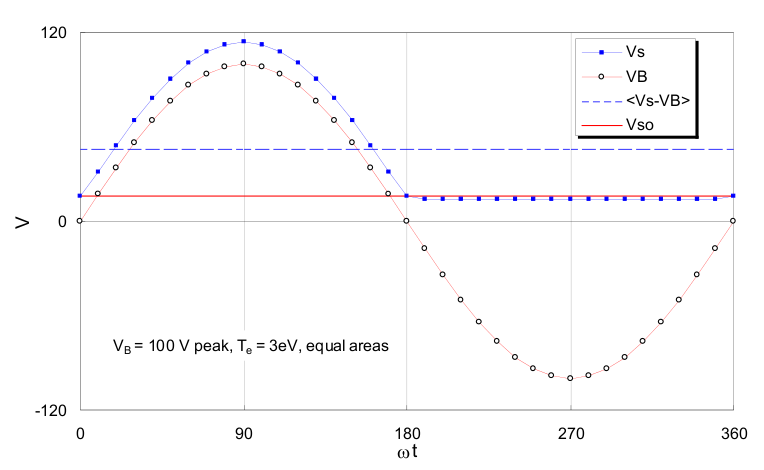
\includegraphics[width=120mm]{sheathdrop.png}
  \caption{Průběh potenciálu v plazmatu při rf výboji. Vs - plazmový potenciál, VB - napětí na rf elektrodě, Vso - plazmový potenciál při nulovém napětí, <Vs-VB> - průměrný plazmový potenciál při rf napětí. Obrázek převzat z \cite{chen2003sheet}.}
  \label{sheat}
\end{figure}


Pokud je navíc rf elektroda menší než uzemněná plocha, byl by celkový tok iontů na každou elektrodu rozdílný. Celkový stejnosměrný proud v obvodu je pro často využívané uspořádání s blokovacím kondenzátorem (obrázek \ref{reaktor}) ovšem nulový. Proto musí být tok iontů na obě dvě elektrody stejný. Aby byla dosažena rovnováha, vzniká na menší rf elektrodě záporné napětí, které se nazývá samopředpětí $U_b$ \cite{liebermanselfbias}.

\begin{figure}
  \centering
  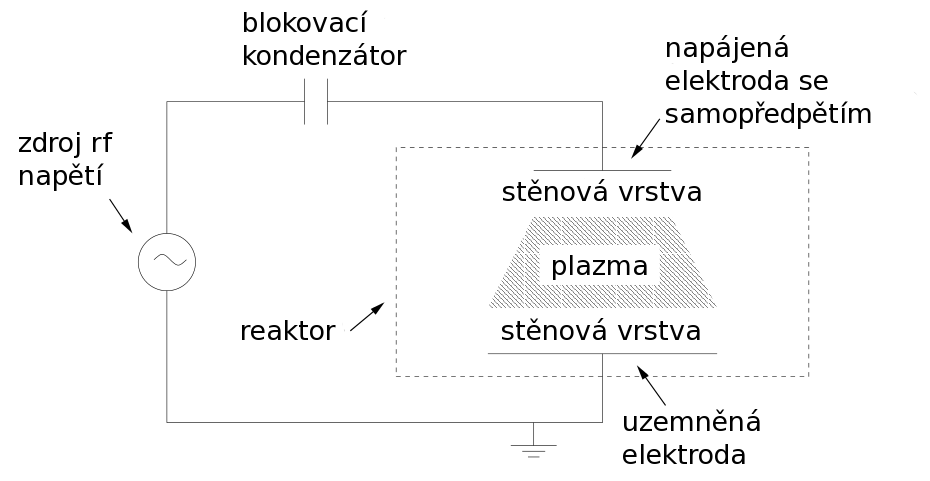
\includegraphics[width=140mm]{reaktor.png}
  \caption{Zjednodušené schéma zapojení reaktoru. Obrázek převzat z \cite{lenkadizertace}.}
  \label{reaktor}
\end{figure}




\chapter{Optické metody měření tenkých vrstev}
Elipsometrie a spektrofotometrie jsou velmi užitečné nedestruktivní metody pro charakterizaci tenkých vrstev. Lze je mimo jiné použít k získání informací o tloušťce vrstvy, optických konstantách a drsnosti povrchu. Nicméně měřená data nejsou zajímavá sama o sobě (výjimkou je propustnost v infračervené oblasti, kde jsou absorpční píky viditelné již přímo z naměřených dat). Užitečné informace, jako je tloušťka vrstvy a optické konstanty, určíme až modelováním vrstvy vzorku a požadované výsledky poté získáme nafitováním naměřených dat do modelu pomocí numerických metod. Je zřejmé, že způsob, jakým je provedena analýza dat, je klíčový a nevhodné modelování může často vést k bezcenným výsledkům \cite{tompkins}.




\section{Elipsometrie}
Princip elipsometrie spočívá ve studiu změn polarizačního stavu světla po odrazu od zkoumaného vzorku. Tato změna se obvykle vyjadřuje jako tzv. elipsometrický poměr $\hat{\rho}$, který je definován jako:
\begin{equation} \hat{\rho} = \frac{\hat{r}_{pp}}{\hat{r}_{ss}} \;\;\; \mathrm{nebo} \;\;\; \hat{\rho} = \frac{\hat{t}_{pp}}{\hat{t}_{ss}} \mathrm{,}\label{elpomer}\end{equation}
kde $\hat{r}_{ss}$ a $\hat{r}_{pp}$ jsou Frenelovy koeficienty odrazu a $\hat{t}_{ss}$ a $\hat{t}_{pp}$ jsou Frenelovy koeficienty průchodu pro s a p polarizovanou vlnu. Vztah (\ref{elpomer}) platí za předpokladu, že normalizovaná Jonasova matice systému je diagonální, tj. $\hat{r}_{sp} = \hat{r}_{ps} = 0$ a $\hat{t}_{sp} = \hat{t}_{ps} = 0$. Elipsometrický poměr můžeme vyjádřit pomocí elipsometrických parametrů $\Psi$ (azimut) a $\Delta$ (fázový posun) jako:
%
\begin{equation} \hat{\rho} = \tan{\Psi} \; e^{i\Delta} \mathrm{.}\end{equation}
%
Při fázově modulované elipsometrii používáme elipsometr v konfigurace polarizátor -- kompenzátor -- substrát -- analyzátor nebo polarizátor -- substrát -- kompenzátor -- analyzátor, přičemž polarizátor, kompenzátor a analyzátor jsou vůči sobě v zafixovaných pozicích. Fázové zpoždění kompenzátoru $\delta$ je periodickou funkcí času. Pokud azimutální úhly použitých komponent splňují vztahy $P - C = \pm \pi/4$, $C=0, \pi/2$ a $A = \pm \pi/4$, pak pro světelný tok $I$ na detektoru můžeme psát:
%
\begin{equation} I(t) \propto 1 + I_s \sin{\delta(t)} + I_c \cos{\delta(t)} \mathrm{.}\end{equation}
%
Fourierovskou analýzou periodického signálu $I(t)$ jsou získány přidružené elipsometrické parametry $I_\mathrm{s}$ a $I_{\mathrm{c}}$, pro které platí:
\begin{equation} I_\mathrm{s} = \sin{2\Psi} \sin{\Delta} \mathrm{.}\end{equation}
$I_{\mathrm{c}}$ záleží na konfiguraci komponent, pokud je $P - C = A = \pi/4$ a $ C = 0 $, jedná se o~takzvanou konfiguraci II:
\begin{equation} I_\mathrm{cII} = \sin{2\Psi} \cos{\Delta} \mathrm{,}\end{equation} 
při $P - C = A = C = \pi/4$ se jedná o takzvanou konfiguraci III \cite{ohlidal2000}:
\begin{equation} I_\mathrm{cIII} = \cos{2\Psi} \mathrm{.}\end{equation}

\section{Viditelná a UV spektroskopická reflektometrie}
Při spektroskopické reflektometrii měříme spektrální závislost poměru intenzity dopadajícího a odraženého světla. Spektrofotometr může být buď jednokanálový, nebo dvoukanálový. V této práci byl používán dvoukanálový spektrofotometr, proto se bude tato kapitola zabývat právě dvoukanálovou konfigurací. V použitém dvoukanálovém spektrofotometru je jeden zdroj záření, ale poté je paprsek rozdělen na dva kanály a každý kanál má vlastní detektor. První kanál je vzorkový, druhý referenční. Pro měřené intenzity na vzorkovém kanále $I_{s1}$ a referenčním kanále $I_{r1}$ můžeme psát:
\begin{equation} I_{s1} = R_n Z_1 D_{s1} G_n \mathrm{,}\;\;\;\;\;\; I_{r1} = R_r Z_1 D_{r1} G_r \mathrm{,}\end{equation}
kde $R_n$ a $R_r$ jsou odrazivosti vzorků, $Z_1$ je aktuální intenzita zdroje v čase měření, $D_{s1}$ a $D_{r1}$ citlivost detektoru v čase měření a $G_s$,$G_r$ jsou geometrické faktory pro jednotlivé kanály, které zahrnují například různé polohy (naklonění) vzorků a různé technické provedení obou kanálů (například polopropustné zrcadlo nemusí propouštět na oba dva kanály stejně světla). 

Je vidět, že již z těchto dvou měření, za předpokladu znalosti odrazivosti jednoho ze~vzorků, by šla určit odrazivost druhého. Problém je, že ve výsledku by vystupoval poměr $G_s/G_r$ a geometrické faktory, které se na obou kanálech mohou značně lišit, nejdou určit. Proto se provádí měření dvě. Poprvé je na vzorkový kanál umístěn vzorek normálový se známou odrazivostí. Na referenční kanál je umístěn vzorek referenční, můžeme použít libovolné zrcadlo. Při druhém měření umístíme na vzorkový kanál vzorek, který chceme změřit, a druhý kanál ponecháme beze změny. Pro naměřené intenzity při druhém měření platí:
\begin{equation} I_{s2} = R_s Z_2 D_{s2} G_s \;\;\;\;\;\; I_{r2} = R_r Z_2 D_{r2} G_r \mathrm{,}\end{equation}
kde $R_s$ je odrazivost vzorku, který chceme změřit, $G_s$ je geometrický faktor měřeného vzorku, index 2 u ostatních veličin značí druhé měření. Zkombinováním všech rovnic získáme \cite{necas}:
\begin{equation}  \displaystyle\frac{ \displaystyle\frac{I_{s2}}{I_{r2}} }{ \displaystyle\frac{I_{s1}}{I_{r1}} } = \frac{R_s}{R_n} \frac{G_s}{G_n}\frac{D_{s2}}{D_{s1}}\frac{D_{r2}}{D_{r1}}\mathrm{.}\end{equation}

Ve výsledném vztahu nevystupují fluktuace zdroje a geometrický faktor na druhém kanálu, protože byl pro obě měření stejný. Poměr $G_s/G_n$ je blízký jedné, protože se jedná o stejný kanál, pouze vzorky vzorky jsou různé. Proměnlivé citlivosti detektorů se dají vykompenzovat vyšším počtem měření. Pokud $G_s = G_n$ a citlivost detektorů se v čase nemění, získáme jednoduchý vzorec:
\begin{equation}R_s = R_n \frac{ \displaystyle\frac{I_{s2}}{I_{r2}} }{ \displaystyle\frac{I_{s1}}{I_{r1}} } \mathrm{.}\end{equation}



\section {Infračervená absorpční spektroskopie}
Infračervené (IR) spektrum obsahuje absorpční píky, které odpovídají frekvenci vibrací molekul a chemických skupin, jež tvoří materiál. Protože každá látka má své unikátní složení a prostorovou strukturu, žádné dvě látky nemohou produkovat stejné IR spektrum. Z IR spektroskopie tedy můžeme podle polohy píků identifikovat (kvalitativně) složení vzorku. Kromě toho velikost píků ve spektru obsahuje i informaci o množství dané sloučeniny nebo skupiny.

Infračerveným zářením bývá nazýváno elektromagnetické záření o vlnočtech 250--12500\,cm$^{-1}$ (pro charakterizaci infračerveného záření je zvyk používat vlnočet v centimetrech, místo vlnové délky nebo energie). V dalším zkoumání se zaměříme na tzv. střední IR oblast mezi 250--5000\,cm$^{-1}$. Záření o této vlnové délce nemá dostatečnou energii k excitaci valenčních elektronů v atomech, ale jeho energie je dostatečná pro změnu stavu molekuly, rotačního nebo vibračního. Samotné rotační a vibrační stavy jsou kvantovou záležitostí a pro jejich úplný popis potřebujeme kvantovou mechaniku. Pro zjednodušený popis a schéma různých druhů vibrací se ale běžně používá klasická mechanika, kde o molekule uvažujeme jako o harmonickém oscilátoru.

Cílem absorpční spektroskopie je změřit spektrální závislost absorpce. Nejjednodušší způsob jak toto změřit, je použít záření ze spojitého zdroje světla, monochromátorem propustit pouze část světla o určité vlnové délce, měřit kolik světla je absorbováno a měření opakovat pro celé spektrum měřených vlnových délek. 

Nevýhodou tohoto postupu je jeho značná časová náročnost. Fourierovská infračervená spektroskopie (FTIR\footnote{Fourier transform infrared (spectroscopy)}) je způsob, jak rychle získat stejné informace. Místo ozařování vzorku pouze monochromatickým světlem, při FTIRu se místo mono\-chromátoru používá Michelsonův interferometr. V něm dochází k interferenci světla a vznik\-ne takzvaný interferogram. Ten měníme pohybem zrcadla v interferometru. Výsledek se na počítači fourierovskou transformací převede na spektrální závislost absorpce.



%\chapter{Modely tenkých vrstev}
%
%
%\section{PJDOS model}
%.. \cite{franta} 
%
%TODO: asi trochu rozvést ten úvod, zjistit co je zač zbytek parametrů, nebo celou kapitolu úplně zrušit...
%
%Modelové parametry:
%
%\begin{tabular}{|l||c|}
%  $Q_f$ & \\
%  $E_g$ & Šířka zakázaného pásu [eV] \\
%  $E_n$ & Maximální energie mezipásového přechodu [eV]\\%
%
%  $d^e$ & tloušťka vrstvy na elipsometrii [nm] \\
%  $d^s$ & tloušťka vrstvy na odrazivosti [nm] \\
%
%  $Q_l$ &\\
%
%  $Q_{Gx}$ & výška absorbční Gaussovy funkce \\
%  $E_{Gx}$ & poloha absorbční Gaussovy funkce \\
%  $B_{Gx}$ & pološířka absorbční Gaussovy funkce \\
%
%parametry instrument correction
%  $d_s$ & tloušťka substrátu [nm] \\
%  $F_E$ & \\
%  $F_R$ & \\
%  $F_R^2$ & \\
%\end{tabular}


\chapter{Experiment}



\section{Depozice tenkých vrstev}
\subsection{Popis reaktoru R2}
Jedná se o válcový ocelový reaktor s planárními elektrodami. Jeho vnitřní průměr je 490\,mm a má výšku 246\,mm. Horní i dolní elektroda mají kruhový tvar. Průměr horní elektrody je 380\,mm, průměr dolní 400\,mm. Horní elektroda je uzemněná. Plyny pro depozici jsou do reaktoru přiváděny přes horní elektrodu, ve které jsou pro tento účel umístěny otvory, které jsou umístěny středově symetricky v kru\-hu o průměru 180\,mm. Vzorek je umístěn na dolní elektrodě, kam je také přiváděno vysokofrekvenční napětí. Jako zdroj byl použit rf (13,56\,MHz) generátor Cesar 133 firmy Dressler.


Tlak v aparatuře je měřen kapacitronem Leybold. Průtoky plynů do reaktoru jsou regulovány průtokoměry Hastlings. Kapalný HMDSO do reaktoru přivádíme přes jehlový ventil. Přesný průtok HMDSO $Q_{\mathrm{HMDSO}}$ vypočítáme na počítači pomocí změn tlaku v reaktoru podle vzorce:
\begin{equation} Q = \frac{\Delta p}{\Delta t} \frac{V}{p_{atm}} \end{equation}
kde $V$ je objem reaktoru a $p_{atm}$ atmosférický tlak. Takto můžeme také ověřit správnou funkci průtokoměrů nebo vakuovou těsnost reaktoru. 


\subsection{Depoziční podmínky}

Všechny měřené vrstvy byly připraveny v reaktoru R2 ve vysokofrekvenčním kapacitně vázaném výboji. Depoziční podmínky vrstev jsou shrnuty v tabulce \ref{podminky}. Zatímco tlak $p$, výkon $P$ a čas $t$ depozice jsou nezávislé depoziční podmínky, samopředpětí $U_b$ závisí na tlaku a na výkonu. Platí přibližně $U_b \sim P^{\frac{1}{2}}$. Vrstvy byly deponovány na křemíkový substrát Si19 o~tloušťce 381$\pm$21\,$\mathrm{\mu}$m s odporem 5,0--9,0\,$\mathrm{\Omega}$\,cm$^-1$.

Všechny kusy křemíkového substrátu byly před depozicí čištěny v ultrazvukové lázni po dobu 10\,minut ve směsi isopropylalkoholu a cyklohexanu v poměru jedna ku jedné. Poté byly osušeny proudem vzduchu a umístěny na elektrodu do reaktoru.

Dalším krokem bylo čištění plazmatem. Pro vrstvy A31--34 bylo použito O$_2$ plazma s průtokem 10\,sccm a výkon zdroje byl nastaven na 100\,W, tlak v reaktoru 5\,Pa. Celková doba čištění byla 60\,minut. Vzorek A38 nebyl plazmově čištěn. V případě A39--A43 byl místo kyslíku použit argon. Parametry výboje byly podobné jako v případě A31--A34, tj. průtok 10\,sccm, výkon 100\,W a tlak 5,5\,Pa. Délka čištění byla ale pouze 5\,minut. 

\begin{table}
 \centering
 \begin{tabular}{|l|c|c|c|c|c|c|c|}
  \hline
  {\bf Vrstva} & {\bf Q$_{\mathrm{HMDSO}}$} & {\bf Q$_\mathrm{\ce{O2}}$} & {\bf \%HMDSO} & {\bf $P$ [W]} & {\bf $U_b$ [V]} & {\bf $p$ [Pa]} & {\bf $t$ [min]} \\
   & {\bf [sccm]} & {\bf [sccm]} & & & & & \\
  \hline \hline

   A31 & 4 & 0  & 100 & 50  & 75  & 5,0  & 10 \\
   A32 & 4 & 0  & 100 & 100 & 134 & 5,0  & 10 \\
   A33 & 4 & 0  & 100 & 100 & 74  & 10,0 & 5  \\
   A34 & 4 & 0  & 100 & 50  & 82  & 2,5  & 10 \\
   A38 & 4 & 20 & 17  & 200 & 157 & 6,0  & 15 \\
   A39 & 4 & 20 & 17  & 300 & 192 & 6,0  & 15 \\
   A40 & 2 & 10 & 17  & 300 & 215 & 4,5  & 15 \\
   A41 & 2 & 22 & 8   & 300 & 180 & 6,2  & 15 \\
   A42 & 1 & 12 & 8   & 300 & 360 & 4,2  & 30 \\
   A43 & 1 & 12 & 8   & 300 & 300 & 3,9  & 60 \\
  \hline
 \end{tabular}
 \caption{Depoziční podmínky, Q$_\mathrm{{HMDSO}}$ je průtok HMDSO, Q$_\mathrm{\ce{O2}}$ je průtok kyslíku, $P$ je výkon, $U_b$ je samopředpětí, $p$ je tlak a $t$ je délka depozice}
\label{podminky}
\end{table}

\subsection{Optické měřící přístroje}

\subsubsection{Bruker VERTEX 80v}
VERTEX 80v je vakuový FTIR spektrofotometr využívající Michelsonova interferometru, jehož zrcadlo kmitá na vzduchovém polštáři. Byl použit speciální nástavec, jež umožňuje správné měření propustnosti. Vzorek byl při měření umístěn svisle na držáku v komoře, ze které byl vyčerpán vzduch na 2,51\,hPa. Vakuum je důležité kvůli eliminování vlivu prostředí a atmosférické vlhkosti. Udávané spektrální rozlišení spektrometru je méně než než 0,2\,cm$^{-1}$. Infračervený spektrofotometr VERTEX 80v obsluhujeme pomocí programu OPUS \cite{vertex}. 

\begin{figure}
  \centering
  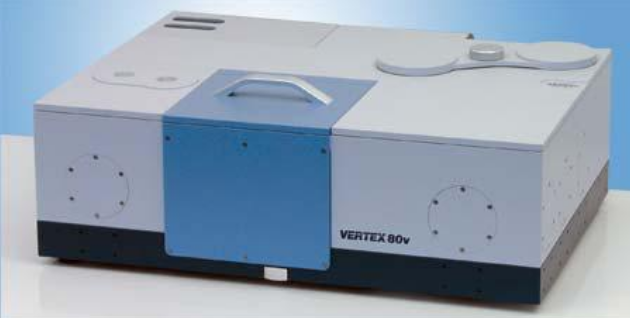
\includegraphics[width=120mm]{vertex80v.png}
  \caption{Spektrofotometr Bruker VERTEX 80v.}
  \label{verteximg}
\end{figure}

\subsubsection{LAMBDA 45 UV/VIS}
LAMBDA 45 je spektrofotometr od firmy PerkinElmer určený pro měření na vzorcích tekutin, regulační zkoušky vyžadující proměnlivé rozlišení a vzorky, které vysoce rozptylují světlo. Je vybaven monochromátorem, který omezuje rozptyl světla. Jeho měřící rozsah je v rozmezí 190--1100\,nm. Zdrojem světla pro viditelnou a blízkou UV oblast je halogenová lampa, pro UV oblast lampa deuteriová. Udávaná přesnost vlnové délky je $\pm$ 0,1\,nm. Jedná se o dvoukanálový spektrofotometr, tj. svazek světla je rozdělen na dva kanály, jeden jde na referenční vzorek (zrcadlo), kde se zjišťuje aktuální intenzita paprsku, a druhá část dopadá na vzorek. Každý kanál má svůj detektor. Tento spektrofotometr poskytuje vysokou stabilitu, přesnost a opakovatelnost měření \cite{lambda}.

\begin{figure}
  \centering
  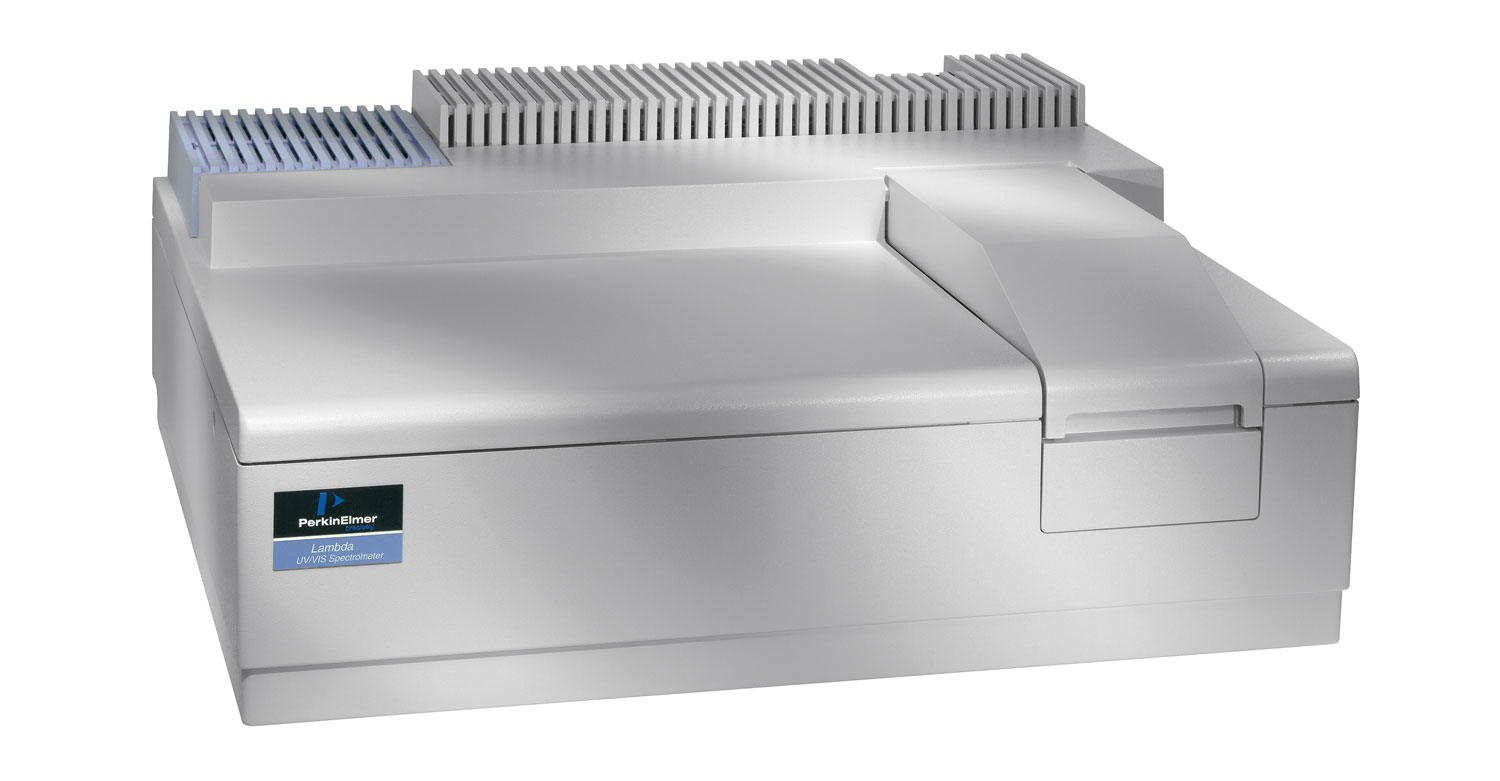
\includegraphics[width=120mm]{LAMBDA.jpg}
  \caption{Spektrofotometr LAMBDA 45 UV/Vis.}
  \label{lambdaimg}
\end{figure}

\subsubsection{Jobin-Yvon UVISEL}
Elipsometr Jobin-Yvon UVISEL je schématicky znázorněn na schématu \ref{fig:elipsometrimg}.  Měřící rozsah tohoto přístroje je od 190\,nm do 2000\,nm. Hlavy elipsometru jsou umístěny na goniometru, měření může být tudíž prováděno pod různými úhly. Běžně se měří úhly dopadu 55$^\circ$, 60$^\circ$, 65$^\circ$, 70$^\circ$ a 75$^\circ$. Jedná se o fázově modulovaný elipsometr. Měření probíhá tak, že z lampy L vychází chromatické nepolarizované světlo, které poté jde přes polarizátor P, kde dojde k jeho lineární polarizaci, odráží se od vzorku a přes kompenzátor C a analyzátor A a monochromátor dopadá na detektor D.


\begin{figure}
  \centering
  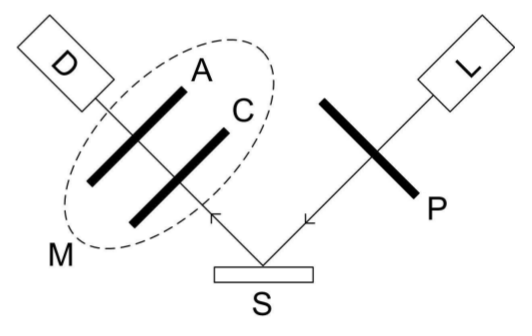
\includegraphics[width=120mm]{schema-elipsometru.png}
  \caption{Schéma elipsometru UVISEL (P--polarizátor, C--kompenzátor, D--detektor, L--lampa, M--modulátor, A--analyzátor, S--substrát), obrázek převzat z \cite{fialova2009}.}
  \label{fig:elipsometrimg}
\end{figure}

\subsection{Zpracování dat}
\subsubsection{IR propustnost}
Každý vzorek na FTIR byl měřen čtyřikrát a po každém měření otočen o 90 stupňů (každé jednotlivé měření se skládalo ze 100 skenů). Na začátku a na konci měření byl změřen tzv. background, tj. referenční signál bez přítomnosti vzorku. Relativní propustnost vrstvy se získá vydělením propustnosti vrstvy na substrátu propustností samotného substrátu $T_{rel} = T / T_{Si}$. Propustnost vrstvy se substrátem byla získána jako aritmetický průměr z výše zmíněných čtyř měření, vydělený průměrem referenčního signálu na začátku a na konci měření. Stejný proces se provedl i pro každý samotný substrát (před depozicí), čímž se získala propustnost substrátu $T_{Si}$. Od tohoto postupu, tedy přeměření každého jednotlivého vzorku před depozicí a po depozici, si slibuji vyšší přesnost měření oproti pouze jednomu měření substrátu pro všechny vrstvy. Data jsem zpracovával v programu QtiPlot (linuxový klon programu Origin). Absorpční píky byly hledány v tabulkách \cite{mayo} a v dřívějších pracích o podobných vrstvách \cite{vasek, zajickova2007b}.

\subsubsection{Elipsometrie a odrazivost}
Pro fitování dat z elipsometrie a odrazivosti byl používán program Daniela Franty xviewerAD. Byl použit PJDOS model, což je disperzní model neuspořádané pevné látky, který parametrizuje společnou hustotu stavů. Tento model umožňuje získat parametry úzce souvisejí s elektronovou strukturou materiálů \cite{franta}.

Program xviewerAD potřebuje data na vstupu ve speciálních formátech, proto bylo potřeba výsledky měření prvně zpracovat. Data z elipsometrie byla nejprve převedena pomocí skriptu "jy-rename.py -d" do kompatibilního formátu a dále byly v programu "ell" vyexportovány do jediného souboru p.dat. Data z odrazivosti bylo také třeba upravit do kompatibilní podoby. To bylo provedeno příkazem "spec *.SP", který vzal všechna data z~měření odrazivosti s koncovkou SP (většinou 5-8 měření) a zapsal je do souboru R.dat. 

Při fitování bylo potřeba se vypořádat s množstvím problémů. Hlavní problém, který se objevil během zpracování dat, byl ten, že fitovaná křivka špatně seděla na měření odrazivosti, především pak na UV konci spektra. Tento problém byl zapříčiněn několika faktory. 

Prvním faktorem byl znečištěný křemíkový normál odrazivosti. To bylo způsobeno tím, že použitý křemík byl používán dlouhou dobu pro mnoho měření a časem se ušpinil. Ve výsledku odrážel méně než měl, a proto odrazivost vzorku vyšla vyšší, mnohdy i značně přes 100\,\% (toto se opět projevovalo hlavně v UV). Tento problém byl eliminován opětovným proměřením vzorků s čistým normálovým křemíkem. 

Druhý problém byl v samotném vyhodnocování dat. Měření z elipsometrie totiž obsahují přibližně desetkrát více bodů než měření z odrazivosti. Z toho plyne, že data z~elipsometrie mají mnohem větší váhu pro celý fit. 

Poslední faktor je ten, že elipsometr měří lineárně podle energií a spektrofotometr LAMBDA 45 lineárně podle vlnové délky a až poté dojde k~přepočtu na energie v elektronvoltech. Z toho důvodu jsou poté data z odrazivosti hustá na~jednom konci spektra a řídká v UV oblasti, které má tím pádem malou váhu pro celý fit. Pro částečné řešení problému s rozdílnou vahou dat byly při vyhodnocování vynásobeny data z odrazivosti faktorem 10.


\section{Parametry fitu}

\begin{table}[b]
 \centering
 \begin{tabular}{|c|c|c|c|c|c|}
  \hline
  {\bf Vrstva} & {\bf $d_e$ [nm]} & {\bf $d_r$ [nm]} & {\bf $E_g$ [eV]} & {\bf $E_h$ [eV]} & {\bf $\chi$} \\
   \hline \hline
   A31 & 278 & 278 & 8,1  & 16,2 & 4,91 \\
   A32 & 473 & 471 & 6,5  & 24,0 & 2,93 \\
   A33 & 290 & 292 & 6,4  & 23,5 & 2,81 \\
   A34 & 269 & 272 & 6,5  & 20,0 & 1,95 \\
   A38 & 620 & 646 & 7,8  & 19,4 & 2,70 \\
   A39 & 716 & 718 & 8,0  & 20,2 & 3,90 \\
   A40 & 395 & 386 & 6,7  & 24,3 & 3,16 \\
   A41 & 372 & 374 & 8,4  & 17,7 & 2,98 \\
   A42 & 426 & 427 & 8,2  & 21,4 & 2,97 \\
   A43 & 867 & 865 & 8,7  & 22,0 & 3,34 \\
   % last update 10.5.2011 11:00
  \hline
  \end{tabular}
  \caption{Některé fitované parametry, $d_e$ je tloušťka vrstvy na elipsometrii , $d_r$ je tloušťka vrstvy na odrazivosti, $E_g$ je šířka zakázaného pásu, $E_h$ je maximální šířka mezipásových přechodů a $\chi$ udává jak souhlasí experimentální data s fitem}
  \label{fitparameters}
\end{table}


Mezi nejdůležitější parametry patří tloušťka vrstvy. Použitý model počítal s tím, že tyto dvě veličiny nemusejí být pro různá měření vždy stejné, proto byla fitována jak tloušťka na elipsometrii $d_e$, tak tloušťka na odrazivosti $d_r$. Na rozdíl od některých běžně používaných modelů pevné látky, kde většina parametrů není zajímavá sama o sobě, ale pouze jako prostředek k získání dalších výsledků (index lomu, extinkční koeficient atd.), v použitém PJDOS modelu mají všechny parametry svůj fyzikální význam. Jde třeba o parametry vztahující se k elektronové struktuře látky, šířka zakázaného pásu $E_g$ a maximální šířka mezipásových přechodů $E_h$. Další důležitá veličina charakterizující fit je $\chi$. Ta udává míru souhlasu fitované funkce s měřenými daty. Data byla fitována metodou nejmenších čtverců. Celková suma čtverců se získá jako:
%
\begin{equation} S = \sum_m S^m f^m \mathrm{,}\end{equation}
%
kde $S^m$ je parciální suma čtverců pro jednotlivá měření (v tomto případě elipsometrie a odrazivost) a $f^m$ jsou faktory kompenzující rozdílný počet měřených bodů $N^m$ pro jednotlivá měření. Parciální sumy čtverců se spočítají jako:
%
\begin{equation} S^m = \sum_{i=1}^{N^m} (X_i^{exp} - X_i^{th})^2 w_i^m \mathrm{,} \end{equation}
%
kde $X_i^{exp}$ a $X^{th}$ jsou měřené a teoretické hodnoty a $w_i^m$ je inverzní hodnota čtverce odhadované chyby měřených veličin. Pro $\chi$ potom platí \cite{Franta2011}:
%
\begin{equation} \chi = \sqrt \frac{S}{\sum_m f^m N^m} \mathrm{.}\end{equation}  
 
Některé fitované parametry vrstev jsou uvedeny v tabulce \ref{fitparameters}. Je vidět že $d_e$ a $d_r$ se od~sebe mírně liší (někdy i o téměř 30\,nm). To je způsobeno tím, že deponovaná vrstva nemá ve všech místech stejnou tloušťku a přestože jsou vzorky relativně malé a snažil jsem se měřit co nejvíc ve středu vzorku, ne vždy se podařilo změřit stejné místo.





\chapter{Diskuze výsledků}


\section{Chemické složení vrstev}

Ve vrstvách A41--A43, které byly deponovány z 8\,\% HMDSO, je absorpční spektrum nejchudší ze všech měřených vrstev. Na obrázku \ref{fig:A41A43ftir} můžeme vidět 5 hlavních píků. Píky na 450\,cm$^{-1}$, 800\,cm$^{-1}$ a největší pík v oblasti 1000-1100\,cm$^{-1}$ přísluší po řadě kolébavým, deformačním a valenčním vibracím skupiny \ce{Si-O-Si}. Úzký pík na 2340\,cm$^{-1}$ patří skupině \ce{CO2}. Široký pík v oblasti 3300\,cm$^{-1}$ až 3600\,cm$^{-1}$ se ve skutečnosti skládá ze dvou píků patřících volným a vázaným OH skupinám. Můžeme si všimnout menších píků v oblasti kolem 500--700\,cm$^{-1}$. To jsou absorpční píky křemíku, jelikož křemík v této oblasti silně absorbuje a použitá metoda zpracování dat, tj. vydělení propustnosti vrstvy se substrátem propustností samotného substrátu, je pouze zjednodušené řešení dané problematiky. Pro ideální výsledek by bylo potřeba udělat kompletní fit infračervených dat.

\begin{figure}
  \centering
  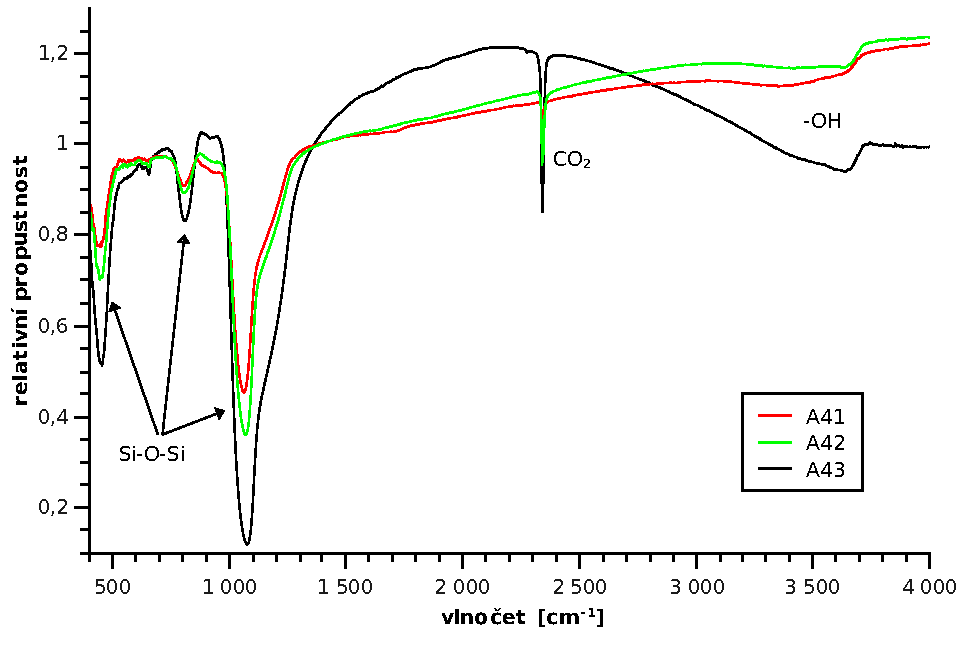
\includegraphics[width=400px]{img/A41A43ftir.pdf}
  \caption{Relativní propustnost vrstev A41, A42 a A43 deponovaných z 100\% HMDSO.}
  \label{fig:A41A43ftir} 
\end{figure}

Vrstvy A39 a A40, které byly deponovány z 17\,\% HMDSO (obrázek \ref{fig:A39A40ftir}), jsou podobné vrstvám A41 až A43, také tu můžeme vidět tři píky příslušející \ce{Si-O-Si} skupině a širokou oblast absorpce OH skupin. Naopak ve vrstvě A39 úplně chybí pík na 2340\,cm$^{-1}$, v A40 je jen nepatrný. Se zvýšeným obsahem HMDSO můžeme naopak pozorovat přítomnost píků příslušejících \ce{CH3} skupinám. V oblasti kolem 2900--3000\,cm$^{-1}$ je to pík odpovídající symetrickým (2900\,cm$^{-1}$) a asymetrickým (2960\,cm$^{-1}$) valenčním vibracím vazby \ce{C-H} ve skupině \ce{CH3}. Další výskyt této skupiny je patrný také z píku na 1275\,cm$^{-1}$, který přísluší symetrickým deformačním vibracím \ce{Si-CH3}. Poslední pík skupiny \ce{CH3} je vidět na vlnočtu 800\,cm$^{-1}$ a jedná se o kolébavou vibraci \ce{CH3} v \ce{Si-(CH3)2}. Poslední výrazný pík je na 2250\,cm$^{-1}$ a přísluší valenčním vibracím skupiny SiH. V oblasti kolem 1300--1800\,cm$^{-1}$ se nachází několik téměř neznatelných píků, které se ale nepodařilo identifikovat kvůli jejich malé velikosti. Pro vrstvu A38 nebyla propustnost v infračervené oblasti zkoumána, protože tato vrstva byla deponována na křemík nevhodný pro toto měření.

\begin{figure}
  \centering
  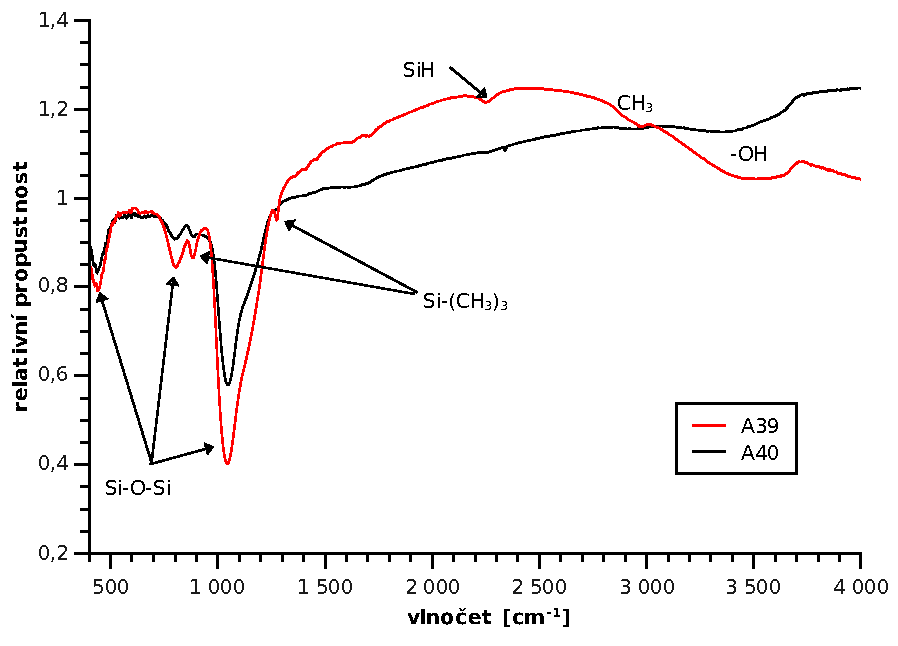
\includegraphics[width=400px]{img/A39A40ftir.pdf}
  \caption{Relativní propustnost vrstev A39 a 40 deponovaných z 17\% HMDSO.}
  \label{fig:A39A40ftir}
\end{figure}

Vrstvy A31--A34, deponované z 100\,\% HMDSO, mají nejzajímavější absorpční spektrum. Oproti předchozím vrstvám úplně chybí píky OH skupiny, valenční pík \ce{Si-O-Si} je výrazně menší a pík na 450\,cm$^{-1}$ příslušející kolébavým vibracím stejné skupiny se ztrácí v šumu. Naopak píky odpovídající symetrickým (2900\,cm$^{-1}$) a asymetrickým (2960\,cm$^{-1}$) valenčním vibracím vazby \ce{C-H} ve skupině \ce{CH3} jsou oproti předchozím vzorkům výrazně znatelnější a ostřejší. Tomu odpovídá přítomnost nových píků spojených právě s~těmito skupinami. Jsou přítomny valenční (800\,cm$^{-1}$ a 840\,cm$^{-1}$) a deformační (1260\,cm$^{-1}$ , 1410\,cm$^{-1}$ ) vibrace skupin \ce{Si-(CH3)_{1,2,3}}. Opět je také přítomen pík na 2250\,cm$^{-1}$ valenčních vibrací skupiny SiH. U vrstvy A32, ale v menší míře i u ostatních vrstev, si můžeme všimnout píku na 1710\,cm$^{-1}$ valenčních vibrací skupiny CO. 

\begin{figure}
  \centering
  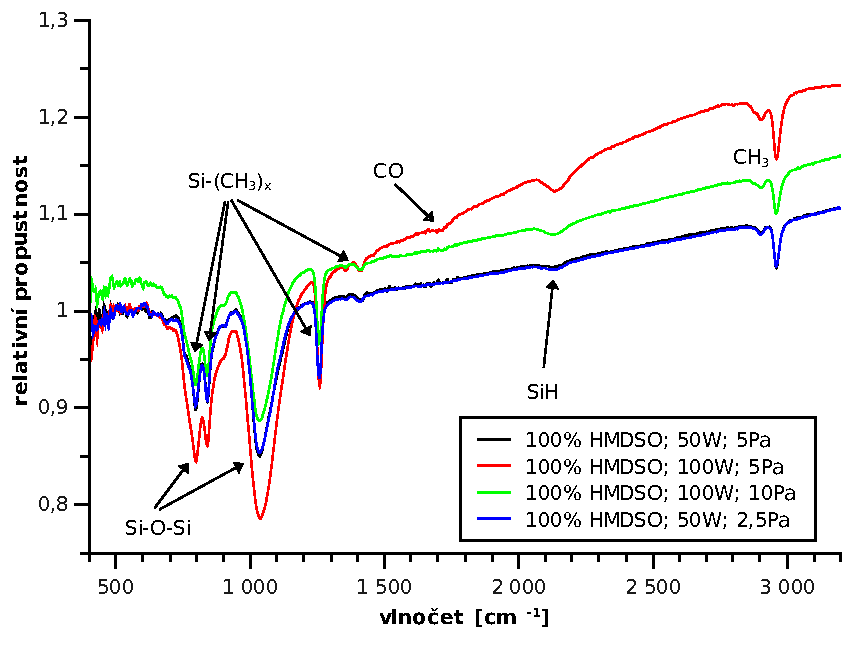
\includegraphics[width=400px]{img/A31A34ftir.pdf}
  \caption{Relativní propustnost vrstev A31, A32, A33 a A34 deponovaných z 8\% HMDSO.}
  \label{fig:A31A34ftir}
\end{figure}

Je zajímavé sledovat posun největšího píku \ce{Si-O-Si}. Pro vrstvy A31--A34 je jeho minimum kolem 1030\,cm$^{-1}$--1040\,cm$^{-1}$, ve vrstvách A39 a A40 je na~1045\,cm$^{-1}$, pro A41 na~1065\,cm$^{-1}$, pro A42 na~1070\,cm$^{-1}$, a konečně ve vrstvě A43 má minimum na 1080\,cm$^{-1}$. Jeho posun je způsoben jednak rostoucím množstvím kyslíku ve vrstvě a také zvyšující se tloušťkou vrstev \cite{trunec2010}. To se skvěle shoduje s depozičními podmínkami a určenou tloušťkou vrstev.


\section{Optické vlastnosti vrstev}


U vrstev deponovaných z 8\% HMDSO byla na vrstvách A42 a A43 ověřována reprodukovatelnost depozice. Obě dvě vrstvy byly deponovány při 300\,W a tlaku kolem 4\,Pa. Jak je vidět z obrázku \ref{fig:A41nA43n}, jejich indexy lomu jsou skutečně téměř totožné. Extinkční koeficient vrstvy A42 je o něco vyšší než u A43, tento rozdíl mezi vrstvami je pravděpodobně způsobem tím, že se nepodařilo vytvořit úplně totožné depoziční podmínky. Vrstva A42 byla deponována za mírně vyššího tlaku a předpětí. Tomu, že s rostoucím tlakem extinkční koeficient roste, odpovídá i srovnání vrstev A42 a A43 s A41. Vrstva A41 je deponována za tlaku 6,2\,Pa a její extinkční koeficient je větší než u A42 a A43. Také index lomu zde roste s tlakem.

\begin{figure}[p]
  \centering
 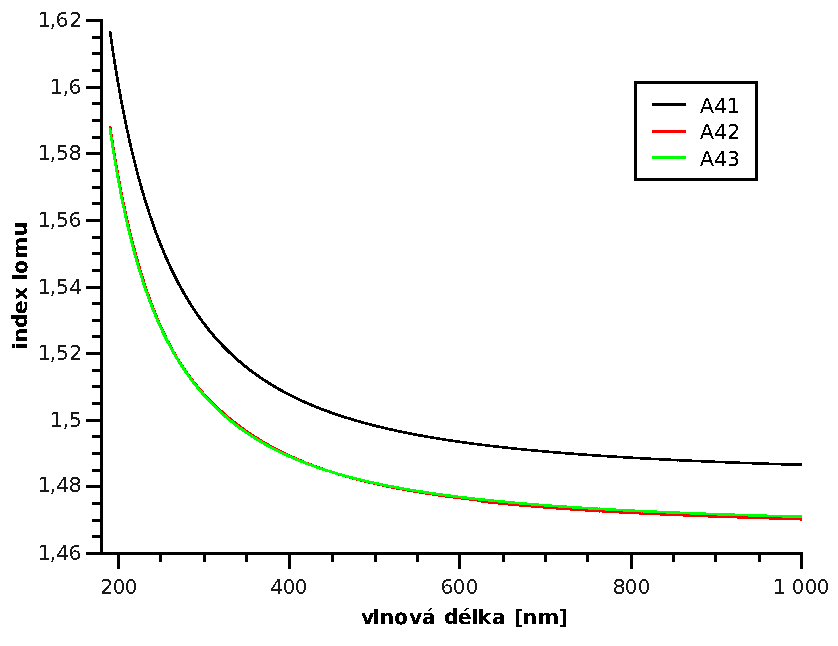
\includegraphics[width=400px]{img/A41nA43n.pdf}
  \caption{Index lomu vrstev A41, A42 a A43 deponovaných z 8\% HMDSO při výkonu 300\,W a tlaku po řadě 6,2\,Pa, 4,2\,Pa a 3,9\,Pa.}
  \label{fig:A41nA43n}
\end{figure}

\begin{figure}[p]
  \centering
  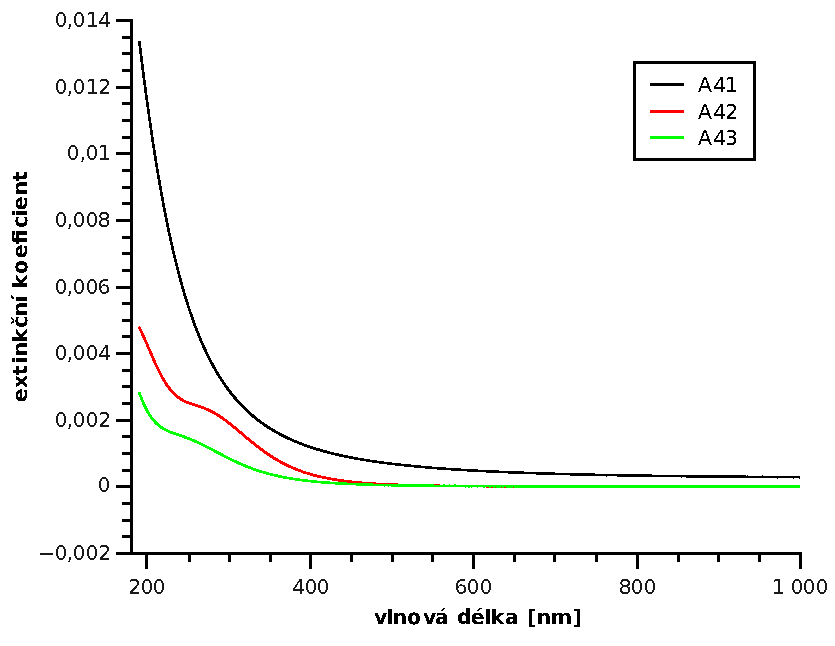
\includegraphics[width=400px]{img/A41kA43k.pdf}
  \caption{Extinkční koeficient vrstev A41, A42 a A43.}
  \label{fig:A41kA43k}
\end{figure}

Na vrstvách A38, A39 a A40 deponovaných z 17\% HMDSO máme poprvé příležitost zkoumat vliv výkonu na optické vlastnosti. Srovnáním indexu lomu (obrázek \ref{fig:A38nA40n}) a extinkčního koeficientu (obrázek \ref{fig:A38kA40k}) vrstev A39 a A40, deponovaných za stejného tlaku (6 Pa) a výkonu 200\,W a 300\,W, můžeme vidět, že index lomu i extinkční koeficient s rostoucím výkonem také rostou. Vrstva A38 má nižší depoziční výkon i tlak než předchozí dvě vrstvy, její extinkční koeficient a index lomu jsou také nižší, což potvrzuje předchozí závěry.

\begin{figure}[p]
  \centering
  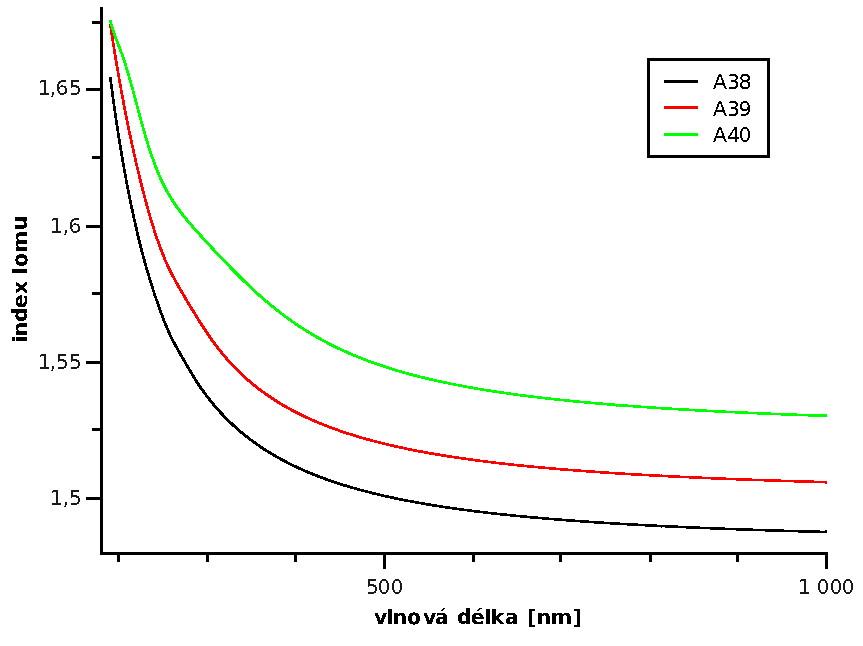
\includegraphics[width=400px]{img/A38nA40n.pdf}
  \caption{Index lomu vrstev A38, A39 a A40 deponovaných z 17\% HMDSO při tlaku po řadě 6\,Pa, 6\,Pa a 4,5\,Pa a výkonu po řadě 200\,W, 300\,W a 300\,W.}
  \label{fig:A38nA40n}
\end{figure}

\begin{figure}[p]
  \centering
  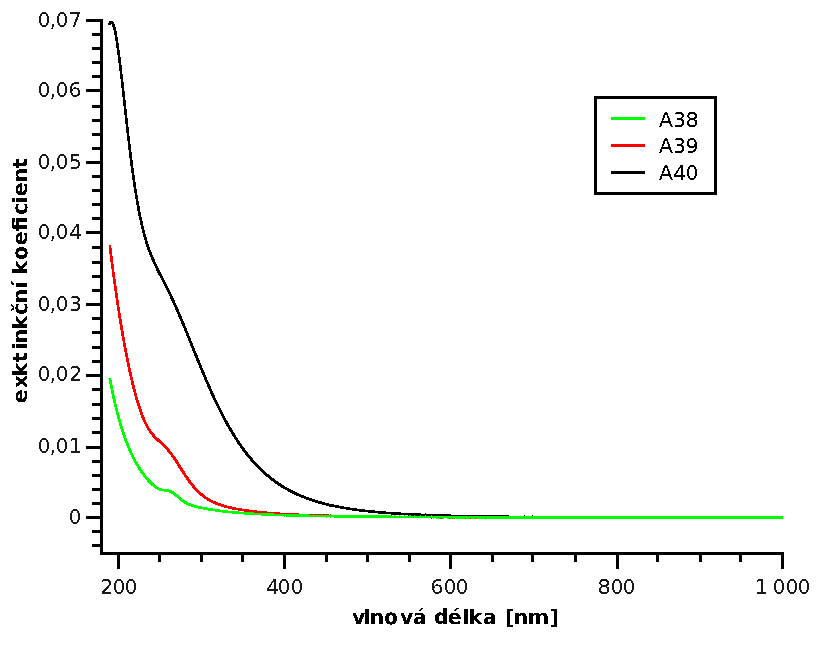
\includegraphics[width=400px]{img/A38kA40k.pdf}
  \caption{Extinkční koeficient vrstev A38, A39 a A40.}
  \label{fig:A38kA40k}
\end{figure}

\begin{figure}[p]
  \centering
  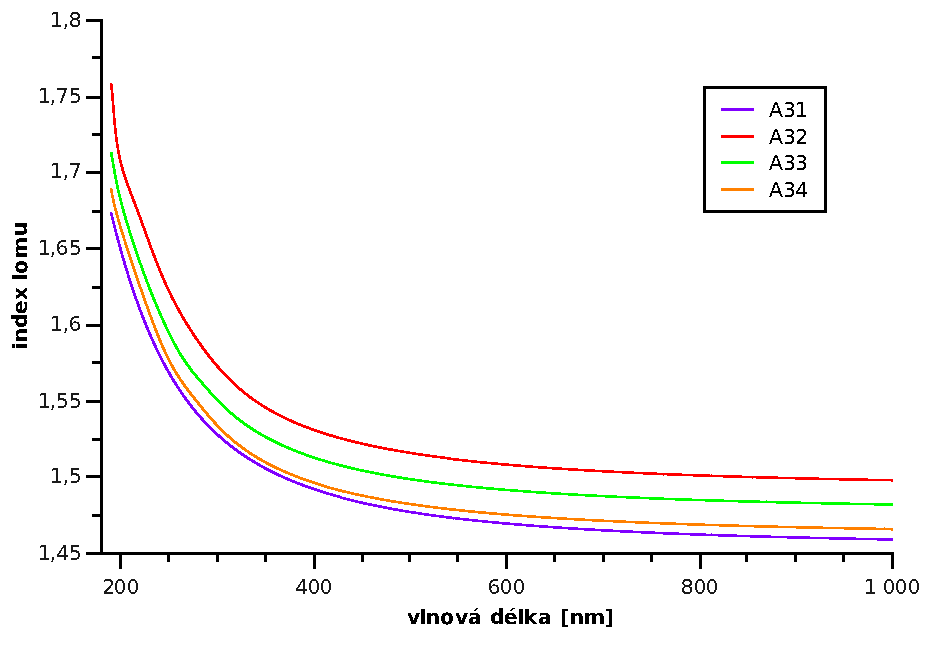
\includegraphics[width=400px]{img/A31nA34n.pdf}
  \caption{Index lomu vrstev A31, A32, A33 a A34 deponovaných z 100\% HMDSO a tlaku po řadě 5\,Pa, 5\,Pa, 10\,Pa a 2,5\,Pa a tlaku po řadě 50\,W, 100\,W, 100\,W a 300\,W.}
  \label{fig:A31nA34n}
\end{figure}

\begin{figure}[p]
  \centering
  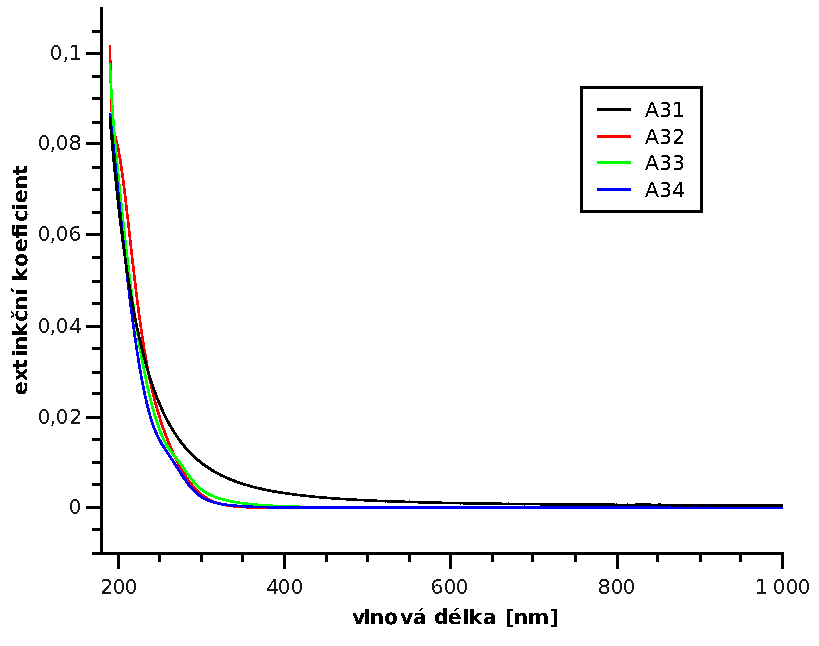
\includegraphics[width=400px]{img/A31kA34k.pdf}
  \caption{Extinkční koeficient vrstev A31, A32, A33 a A34.}
  \label{fig:A31kA34k}
\end{figure}
%\clearpage

U vrstev A31 až A34 deponovaných z 100\% HMDSO je situace poněkud komplikovanější. Pokud zde zkoumáme vliv tlaku na vrstvy vyrobené při stejném výkonu, dojdeme k úplně opačným závěrům. Jak si lze povšimnout na obrázku \ref{fig:A31nA34n}, index lomu vrstvy A31 deponované při výkonu 50\,W a tlaku 5\,Pa je menší než index lomu vrstvy A34 deponované taktéž při výkonu 50\,W, ale při tlaku 2,5\,Pa. Stejný trend můžeme pozorovat i u~vrstev A33 a A32. Obě byly deponovány za stejného výkonu 100\,W, ale index lomu vrstvy A33 je menší než index lomu vrstvy A32, přestože byla deponována za dvojnásobného tlaku (10\,Pa a 5\,Pa). Spektrální závislost extinkčních koeficientů těchto vrstev můžeme vidět na obrázku \ref{fig:A31kA34k}. Je vidět, že je téměř u všech vrstev velmi podobná. Výjimkou je vrstva A31, která má na intervalu 150--500\,nm vyšší extinkční koeficient než ostatní vrstvy. Proč se zrovna vrstva A31 takto liší od ostatních, není bohužel z depozičních podmínek vůbec patrné. 
 


\section{Rychlost růstu vrstev}

\begin{table}[b]
 \centering
 \begin{tabular}{|c|c|c|c|}
  \hline
  {\bf Vrstva} & {\bf tloušťka} & {\bf doba depozice} & {\bf rychlost růstu vrstvy} \\
  {}&{[nm]}&{[min]}&{[nm min$^{-1}$]}\\
   \hline \hline
   A31 & 278 & 10 & 27,8 \\
   A32 & 472 & 10 & 47,2 \\
   A33 & 291 & 5  & 58,2 \\
   A34 & 271 & 10 & 27,1 \\
   A38 & 633 & 15 & 42,2 \\
   A39 & 717 & 15 & 47,8 \\
   A40 & 391 & 15 & 26,1 \\
   A41 & 373 & 15 & 24,9 \\
   A42 & 427 & 30 & 14,2 \\
   A43 & 866 & 60 & 14,4 \\
   % last update 10.5.2011 15:00
  \hline
  \end{tabular}
  \caption{Rychlost růstu vrstev.}
  \label{rychlost}
\end{table}

Dalším cílem této práce je zkoumat vliv depozičních podmínek na rychlost depozice. Přehledně rychlost růstu jednotlivých vrstev shrnuje tabulka \ref{rychlost}. Jelikož byla tloušťka vrstev určována z fitu, je uvedená tloušťka spočítána jako průměr $d_e$ a $d_r$. Je vidět, že rychlost růstu se mezi vrstvami značně liší v závislosti na depozičních podmínkách (tabulka \ref{podminky}). Protože při depozicích bylo cílem vyrobit co nejširší spektrum vrstev s co nejrůznějšími vlastnostmi, depoziční podmínky se výrazně mění od vrstvy k vrstvě. To znemožňuje udělat přesný závěr o vlivu jednotlivých podmínek na růst vrstev. 

Při následujících závěrech bylo předpokládáno, že vrstvy rostou lineárně. Tomu odpovídá i to, že rychlosti růstu vrstev A42 a A43, které měly stejné depoziční podmínky pouze rozdílnou délku depozice, jsou téměř totožné. 

Pro zjištění vlivu tlaku na rychlost depozice jsou porovnávány vrstvy deponované za~stejného výkonu. Vrstvy A41 a A42 byly deponovány při stejném výkonu 300\,W, vrstva A41 je deponována za většího tlaku (6,2\,Pa) než vrstva A42 (4,2\,Pa) a má také větší depoziční rychlost. Stejný trend můžeme pozorovat i při porovnání zbytku vrstev, například A39 s~A40, A31 s A34 a A32 s A33. Vrstvy deponované za vyššího tlaku mají ve všech případech větší rychlost růstu. Nejrychleji rostoucí byla vrstva A33, která byla ze všech vrstev deponována za nejvyššího tlaku (10\,Pa).

Vliv výkonu zkoumáme porovnáním vrstev deponovaných při stejném tlaku. Zde je jasně viditelný růst depoziční rychlosti při zvyšování výkonu. Je to vidět třeba na vrstvách A38 a A39. Obě byly deponovány při tlaku 6\,Pa, ale vrstva A39, která byla deponována při výkonu 300\,W, má vyšší depoziční rychlost než vrstva A38, jejíž depoziční výkon byl jen 200\,W. To stejné platí i pro vrstvy A31 a A32 (50\,W a 100\,W při tlaku 5\,Pa), zde se při zdvojnásobení výkonu depoziční rychlost také téměř zdvojnásobila.

Tyto výsledky se dobře shodují s \cite{yasudaspeed}. Při nízkých výkonech je limitujícím faktorem malý počet radikálů v plazmatu, který se právě od výkonu odvíjí, a se zvyšováním tlaku se depoziční rychlost zvedá jen minimálně. To vidíme dobře na vrstvách deponovaných ze 100\,\% HMDSO při nízkých výkonech, například ve vrstvách A31 a A34, které byly deponovány při výkonu 50\,W, se při zdvojnásobení tlaku v reaktoru rychlost depozice zvýšila o méně než 5\,\%. Při nárůstu výkonu je pro tyto vrstvy pozorovatelné přibližně lineární zvýšení rychlosti depozice. Příkladem tohoto jsou třeba vrstvy A31 a A32.

Při vyšších výkonech je již většina plynů v plazmatu disociována a limitujícím faktorem růstu vrstev se stává dostatek depozičního materiálu v reaktoru, který se odvíjí od tlaku. Například u vrstev A38 a A39 deponovaných při tlaku 6Pa je při zvýšení výkonu o 50\,\% (z 200\,W na 300\,W) pozorován nárůst depoziční rychlosti o 13\,\%. Při dostatečném výkonu se pak zvyšování tlaku projeví velmi výrazným zvýšením depoziční rychlosti. Toto můžeme vidět porovnáním vrstev A39 a A40, případně A42 a A43.

Při porovnávání vrstev deponovaných při různé koncentraci HMDSO jsou také patrné rozdíly při rychlosti růstu. Vrstvy A41 až A43 deponované z 8\% HMDSO mají velmi malé depoziční rychlosti, přestože jsou všechny deponovány za velkého výkonu. Vrstvy deponované při 17\% HMDSO mají při srovnatelných depozičních podmínkách rychlost růstu výrazně větší. Vrstvy A31--A34 deponované z 100\% HMDSO mají obecně rychlost růstu srovnatelnou, případně vyšší, než všechny ostatní vrstvy, přestože byly deponovány při nejnižším výkonu. Z toho plyne, že se vzrůstajícím procentem HMDSO roste depoziční rychlost. Toto je možno vysvětlit tak, že při nízkých koncentracích HMDSO dojde u většiny monomerů k oxidaci v plazmatu.




\chapter{Závěr}
Během této bakalářské práce byly připravovány tenké vrstvy metodou PECVD v doutnavém vysokofrekvenčním kapacitně vázaném výboji ze směsi kyslíku a hexametyldisiloxanu. Na všech vrstvách byla následně změřena odrazivost, elipsometrie a propustnost. Poté byly zkoumány jejich optické vlastnosti v infračervené až ultrafialové části spektra a to především index lomu, extinkční koeficient a absorpce v infračervené oblasti. Z té bylo následně určeno přibližné složení vrstvy. Dále byla zjišťována tloušťka vrstev a některé vlastnosti jejich elektronové struktury. 

V infračervené spektroskopii je s rostoucím procentem HMDSO dobře pozorovatelný přechod od \ce{SiO2} podobných vrstev k organosilikonovým polymerním vrstvám. U vrstev deponovaných z 8\,\% HMDSO pozorujeme pouze píky patřící \ce{Si-O-Si}, \ce{OH} a \ce{CO2} skupinám, u vrstev deponovaných z 100\,\% HMDSO pozorujeme převážně píky skupin \ce{CH3} a \ce{Si-(CH3)_x}. 
Také u studia optických konstant se ukázaly rozdíly ve vlivu depozičních parametrů na optické konstanty mezi organosilikonovými a \ce{SiO2} podobnými vrstvami. Pro vrstvy deponované z 8\,\% HMDSO a 17\,\% HMDSO roste se zvyšujícím se tlakem i výkonem při depozici absorpční koeficient i index lomu. Pro~vrstvy deponované z 100\,\% HMDSO se naopak index lomu s rostoucím tlakem a výkon snižuje. Extinkční koeficient pro tyto vrstvy závisí na depozičních parametrech velmi málo.

Pro rychlost růstu vrstev se jako nejdůležitější parametr ukázal být tlak v reaktoru, s~jehož nárůstem roste i depoziční rychlost. Taktéž s růstem výkonu při depozici roste depoziční rychlost. Také se ukázalo, že rychlost růstu organosilikonových vrstev je obecně vyšší než rychlost růstu \ce{SiO2} podobných vrstev.

Způsoby depozice a optickými metodami charakterizace tenkých vrstev bych se chtěl i nadále zabývat. Z věcí, které se rozsahově do obsahu této práce nevešly, by si podrobnější rozbor jistě zasloužil například problém absorpce v infračervené oblasti. Také by určitě bylo zajímavé vyzkoušet jiné metody zpracování dat než použitý PJDOS model. 




\bibliographystyle{unsrt}
\bibliography{bib-db}
% BibTeX database file

\end{document}
